\chapter{Theory}
\section{The Operational Transconductance Amplifier}

\begin{figure} [H]
\centering
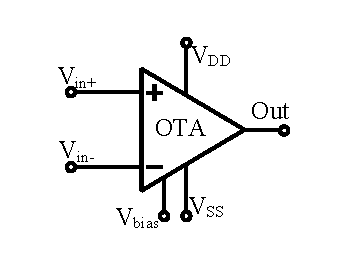
\includegraphics[scale=1]{Figures/System_Level/OTA_Symbol.pdf}
\caption{Symbol of an OTA}
\end{figure}


\subsection{Different Topologies}
\subsubsection{Conventional Current Mirror OTA}
\subsubsection{Super Class AB OTA}
\subsubsection{Folded Cascode OTA}
\section{The Opeartional Amplifier}
\subsection{Miller Compensation OP AMP}
\subsection{OP AMP as a Voltage Buffer}
\section{The Gm/Id Methodology}
